\section{Matrix and Data Normalization for Echo State Networks}
\label{sec:new_methods}

Here we describe several aspects of our ESN implementation that are
unique with respect to previous works.
Additionally we provide some empirical justification for these choices, using
the Lorenz96 model as a testbed \citep{lorenz_predictability_1996}, see
Appendix \cref{subsec:lorenz96} for a description of the datasets generated for these
tests.

Our testing framework follows the general procedure laid out
by \citet{platt_systematic_2022} to evaluate the architecture choices.
For each design choice, we compute the Valid Prediction Time (VPT) of
an ESN model over 100 randomly chosen initial conditions from a test dataset.
VPT is computed as
\begin{linenomath*}\begin{equation*}
    \begin{aligned}
        \text{VPT} &= \argmin_{n} \left\{ \text{NRMSE}(n) > \epsilon \right\} \\
        \text{NRMSE}(n) &= \sqrt{\dfrac{1}{\nstate}\sum_{i=1}^{\nstate}\left(
            \dfrac{\hat{v}_i(n) - v_i(n)}{SD_i}
            \right)^2
        } \, ,
    \end{aligned}
\end{equation*}\end{linenomath*}
where $n$ is a time index, $SD_i$ is the temporal standard deviation of the $i$-th dimension,
computed from the training data, and $\epsilon=0.2$.
To eliminate the dependence of the results on the randomly chosen adjacency and
input matrices, we repeat the process for 10 different adjacency and input
matrix pairs, initialized with different random number generator seeds.
In total, we compare each design choice with a VPT distribution from 1,000 test samples.
We note that we optimize the ESN parameters listed in
\cref{eq:rc-hyperparameters} for each design choice and each random matrix pair,
following the procedure laid out in \cref{sec:optim}.
Of course, these tests are insufficient to definitively prove that these choices
will translate perfectly to the SQG system.
However, we consider this to be a bare minimum test that will catch downright bad
design choices, while saving the computing resources necessary to train an
emulator for larger problems.


\subsection{Input Matrix Scaling}
\label{subsec:input-scaling}

Typically, $\inputmatrix$ is filled with entries
\begin{linenomath*}\begin{equation*}
    \hat{w}_{i,j} \sim \mathcal{U}(-\sigma,\sigma) \qquad
    i = [1, 2, ..., \nhidden], j=[1,2, ..., \ninputstate] \,
\end{equation*}\end{linenomath*}
where $\sigma$ is a hyperparameter that determines the bounds of the uniform
distribution.
Here we found it to be advantageous to normalize the input matrix by the
largest singular value.
That is, we first compute $\hat{\mathbf{W}}_\text{input}$, with elements
\begin{linenomath*}\begin{equation*}
    \hat{w}_{i,j} \sim \mathcal{U}(-1,1) \qquad
    i = [1, 2, ..., \nhidden], j=[1,2, ..., \ninputstate] \, .
\end{equation*}\end{linenomath*}
Then, we set $\inputmatrix$ as
\begin{linenomath*}\begin{equation*}
    \inputmatrix \coloneqq
    \dfrac{\sigma}{\sigma_{max}\left(\hat{\mathbf{W}}_\text{in}\right)}
    \hat{\mathbf{W}}_\text{in} \,
\end{equation*}\end{linenomath*}
where $\sigma_{max}\left(\cdot\right)$ is the largest singular value, and
the hyperparameter $\sigma$ is the desired largest singular value of
$\inputmatrix$.

Our motivation for using this type of normalization is that we found it
necessary to use very wide hyperparameter optimization bounds for $\sigma$ when
using the standard input scaling strategy.
By first normalizing the matrix by the largest singular value compensates for the fact that
the amplitude of the contributions to the reservoir, i.e., the elements of the
vector
\begin{linenomath*}\begin{equation*}
    \mathbf{p} = \inputmatrix \inputstate =
    \begin{pmatrix}
        \mathbf{w}_1^T\inputstate \\
        \mathbf{w}_2^T\inputstate \\
        \vdots \\
        \mathbf{w}_{\nhidden}^T\inputstate
    \end{pmatrix}
\end{equation*}\end{linenomath*}
grow with $\ninputstate$. \todo{this would be the place to talk about variance}
By controlling for this growth, we were able to reduce the optimization search
space and achieve more consistent prediction skill with fewer iterations.

Additionally, we found empirical evidence to suggest that this normalization is
advantageous even for small systems.
\cref{fig:simple-normalization} shows the VPT achieved with
the 20-Dimensional Lorenz96 system (\cref{subsec:lorenz96}), using a variety of
normalization strategies for the input and adjacency matrices.
In \cref{fig:simple-normalization}, the two schemes used for the input matrix
are (1) no normalization (indicated by $c W_{in}$ in
\cref{fig:simple-normalization}) and
(2) normalization by the largest singular vector (indicated by
$\sigma_{max}(W_{in})$).
For a variety of reservoir sizes ($\nhidden$), we found that using the largest
singular vector often performed better, usually by about 0.5~MTU.

\begin{figure}
    \centering
    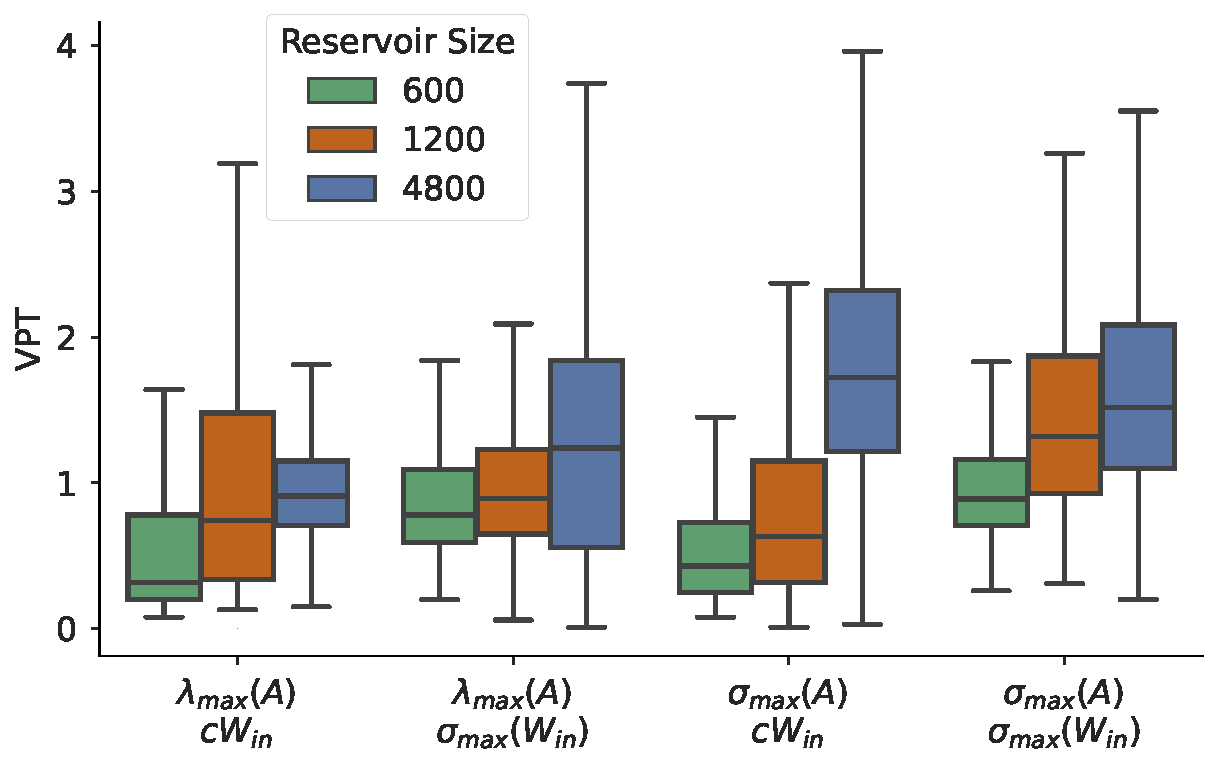
\includegraphics[width=.8\textwidth]{../figures/matrix_normalization.pdf}
    \caption{Valid Prediction Time (VPT) obtained with an ESN, using
        different normalization strategies for the adjacency and input matrices,
        $\adjacency$ and $\inputmatrix$. The normalization used for each matrix
        is indicated as follows:
        $\lambda_{max}(\cdot)$ refers to the largest eigenvalue (i.e.,
        spectral radius),
        $\sigma_{max}(\cdot)$ refers to the largest singular value (i.e.,
        induced 2 norm),
        while $c$ implies that no normalization was used.
        The results are computed with the 20D Lorenz96 system, described in
        \cref{subsec:lorenz96}.
        The boxplots indicate prediction skill from 10 different adjacency and
        input matrices (achieved by changing the random number generator seed),
        with 100 initial conditions randomly sampled from the test dataset for
        each set of matrices.
        The hyperparameters were optimized for each unique matrix pair.
        Color indicates the size of the reservoir used.
    }
    \label{fig:simple-normalization}
\end{figure}

\subsection{Adjacency Matrix Scaling}
\label{subsec:adjacency-scaling}

Typically, the reservoir adjacency matrix is normalized to achieve a desired
spectral radius.
That is, the matrix $\hat{\adjacency}$ is generated with elements
$\hat{a}_{i,j} \sim \mathcal{U}(-1,1)$, where $i,j$ are random indices in order
to satisfy the desired sparsity of the matrix (all other elements are 0).
Then, the $\adjacency$ is set as
\begin{linenomath*}\begin{equation*}
    \adjacency \coloneqq
    \dfrac{\spectralradius}{\lambda_{max}\left(\hat{\adjacency}\right)}
    \hat{\adjacency} \, ,
\end{equation*}\end{linenomath*}
where $\lambda_{max}\left(\cdot\right)$ is the spectral radius, and $\spectralradius$
scales the matrix to achieve the desired spectral radius.
A common guideline is to set $\spectralradius \simeq 1$, as it is hypothesized
that this puts the reservoir on the ``edge of stability'' so that it performs
well in emulating nonlinear systems \citep<e.g., as recommended by>[]{lukosevicius_practical_2012}.
However, as originally described by \citet{jaeger_echo_2001},
the spectral radius provides only a necessary, but insufficient, means to satisfy
the required Echo State Property.
On the other hand, using the largest singular value is a sufficient condition
for satisfying the echo state property.

In our experimentation, we have found a slight benefit from using the largest
singular value to normalize the adjacency matrix.
\cref{fig:simple-normalization} shows that, for fixed input matrix
normalization, using the largest singular value rather than spectral radius
achieves similar and up to $\sim0.3$ longer valid predictions.
While the improvement may seem subtle, we note that using the largest singular value
has the following practical benefit for our python-based implementation:
the singular values can be computed directly on a Graphical Processing Unit
using CuPy \citep{cupy_learningsys2017}, while a general, non-symmetric eigenvalue
decomposition is not readily available.

\subsection{Data Normalization}
\label{subsec:data_normalization}

A key aspect in machine learning is normalizing input data before passing it to
the model.
Experiments from \citet{platt_systematic_2022} showed, however, that the
standard approach to normalizing data
be detrimental to prediction skill.
By ``standard  approach'', we mean
\begin{linenomath*}\begin{equation*}
    v_i(n) = \dfrac{v_i(n) - \bar{v}_i}{SD_i} \qquad i = [1, 2, ...
    \nstate]
\end{equation*}\end{linenomath*}
where $\bar{v}_i, SD_i$ are the mean and standard deviation taken from the
training data for each channel
of input data, indexed by $i$.
The key takeaway from \citet{platt_systematic_2022} is that by using separate
normalization values for each channel, the covarying relationships between the
data are destroyed and so the reservoir cannot learn the true dynamics.
The authors propose to normalize with the average and range of the data,
computed over the length of the training data and over all channels
\begin{linenomath*}\begin{equation}
    v_i(n) = \dfrac{v_i(n) - \bar{\mathbf{v}}}{\max\mathbf{v} - \min\mathbf{v}}
    \qquad i = [1,2, ... \nstate] \, ,
    \label{eq:maxmin}
\end{equation}\end{linenomath*}
Here, we propose to replace the range in the denominator with the
standard deviation computed over all channels and timesteps in the training
data,
\begin{linenomath*}\begin{equation}
    v_i(n) = \dfrac{v_i(n) - \bar{\mathbf{v}}}{SD}
    \qquad i = [1,2, ... \nstate] \, .
    \label{eq:sdnorm}
\end{equation}\end{linenomath*}

\cref{fig:data-norm} compares the prediction skill when these two normalization
strategies are used.
Using the standard deviation normalization as in \cref{eq:sdnorm} leads to an
average VPT increase by two.
We surmise that this improvement is due to the fact that when the data are
normalized by the full range, then all values are in the range $[-1,1]$.
In this case, once the input is mapped into the hidden space, it is more likely
to lie on the linear regime of the $\tanh(\cdot)$ activation function.
While a large enough input scaling could eliminate this problem, it is
apparently not easily obtained during the Bayesian optimization.

\begin{figure}
    \centering
    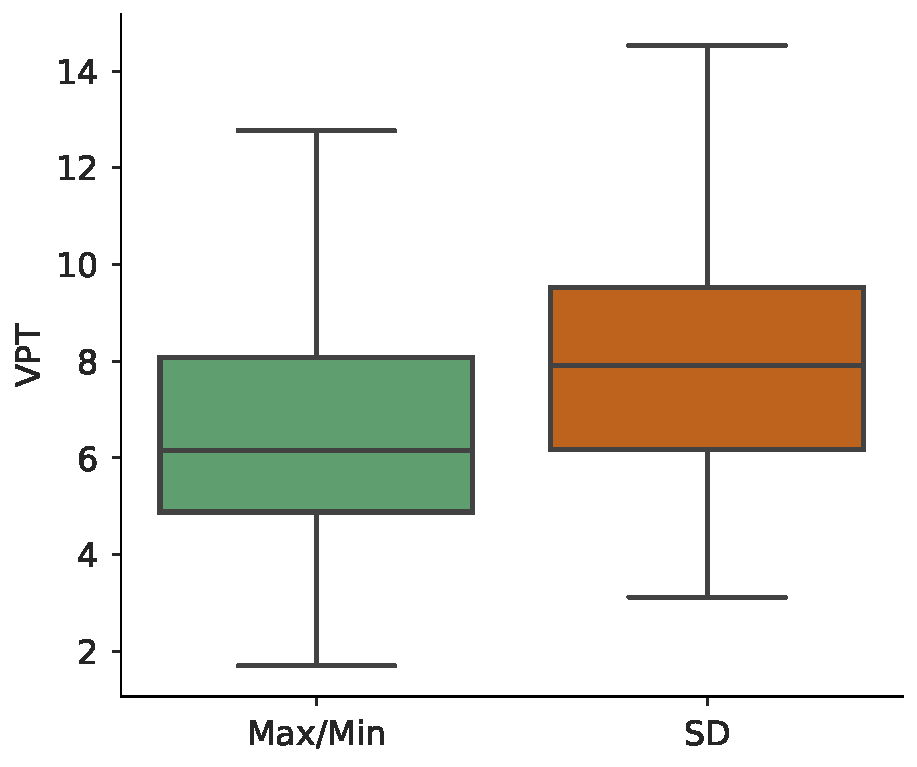
\includegraphics[width=.6\textwidth]{../figures/data-normalization.pdf}
    \caption{Valid Prediction Time (VPT) with an ESN, using the
        Max/Min normalization strategy shown in \cref{eq:maxmin} and standard
        deviation (SD)
        normalization strategy as in \cref{eq:sdnorm}.
        The results are computed with the 6D Lorenz96 system, described in
        Appendix \cref{subsec:lorenz96}.
        The boxplots indicate prediction skill from 10 different adjacency and
        input matrices (achieved by changing the random number generator seed),
        with 100 initial conditions randomly sampled from the test dataset for
        each set of matrices.
        The hyperparameters were optimized for each unique matrix pair.
    }
    \label{fig:data-norm}
\end{figure}

\subsection{Lorenz96 Datasets}
\label{subsec:lorenz96}

The Lorenz96 dataset used for these supplemental experiments were generated by
the following set of equations introduced by \citep{lorenz_predictability_1996},
\begin{linenomath*}\begin{equation*}
    \frac{dx_i(t)}{dt} = x_{i-1}(t)(x_{i+1}(t) - x_{i-2}(t)) - x_i(t) + F \, ,
    \label{eq:lorenz96}
\end{equation*}\end{linenomath*}
where $i=1,2,...,N_{l}$, and the domain is periodic.
$F=8$ is a fixed parameter that generates chaotic dynamics.
We use $N_l = 20$ for the tests in
Appendices \cref{subsec:input-scaling,subsec:adjacency-scaling} and $N_l = 6$ for the tests
in Appendix \cref{subsec:data_normalization}.
Each dataset was generated by stepping the model forward with a 4th order
Runge-Kutta scheme with $\Delta t = 0.01$~Model~Time~Units (MTU).
Each dataset consisted of a 10~MTU spinup period that was discarded, 420~MTU of
training data, a 60~MTU validation period, and a 120~MTU test
period.
Each randomly chosen validation and test trajectory were 1~MTU and 15~MTU,
respectively, and the ESN spinup period was 5~MTU.
